\documentclass[11pt,a4paper]{article}

\usepackage[utf8]{inputenc}
\usepackage[T1]{fontenc}
\usepackage[english]{babel}
\usepackage[a4paper,margin=2.5cm]{geometry}
\usepackage{graphicx}
\usepackage{booktabs}
\usepackage{caption}
\usepackage{hyperref}
\usepackage{amsmath}
\usepackage{enumitem}
\usepackage[natbib=true,style=authoryear,backend=biber]{biblatex}
\addbibresource{references.bib}

\hypersetup{colorlinks=true, linkcolor=black, citecolor=black, urlcolor=blue, pdfusetitle=false, hypertexnames=false}
\usepackage{xcolor}
\newcommand{\TODO}[1]{\textcolor{red}{\textbf{[TODO: #1]}}}


\title{\textbf{Automatic Identification System (AIS): \\
Sampling, Vessel Behaviour, and Traffic Density Analysis}}
\author{
  Filip Pasti, Matriculation No.\ 1091212 \\
  David Gvenetadze, Matriculation No.\ 1090976 \\
  B.Sc.\ Wirtschaftsinformatik, Universit\"at Hohenheim \\[4pt]
  \textit{Team: Team 32} \\
  \textit{Repository: \textcolor{red}{[TODO: paste your AIDAHO GitLab URL]}}
}
\date{Summer Term 2026 \\ Submitted: \today}

\begin{document}

\maketitle
\thispagestyle{empty}
\newpage

\setcounter{page}{1}
https://aidaho-edu.uni-hohenheim.de/gitlab/david.gv/AIDAHO_IDS_THAS_2026

\section{Introduction}
\label{sec:intro}

The Automatic Identification System (AIS) is a maritime tracking technology that
requires vessels above a certain tonnage to continuously broadcast identifying
and positional information over VHF radio \autocite{example_ais_intro}. Each AIS
message falls into one of two broad categories: \emph{static} information, which
changes rarely and includes attributes such as the vessel's name, call sign, flag
state, and physical dimensions; and \emph{dynamic} information, which is updated
every few seconds to minutes and includes the vessel's position, speed over
ground, and course over ground. AIS was originally introduced for collision
avoidance, but the resulting data stream has since become a valuable resource for
studying global shipping patterns, port activity, and inland waterway traffic.

This report analyses an AIS dataset provided through a PostgreSQL/PostgREST
backend maintained by the AIDAHO certificate program. We first provide a
descriptive overview of the database (Section~\ref{sec:data}--\ref{sec:overview}),
then construct and compare two different sampling strategies for the
high-frequency dynamic AIS table (Section~\ref{sec:sampling}), examine the
movement behaviour of individual vessels including an automated ship-lock
detection procedure (Section~\ref{sec:behaviour}), and -- where completed --
relate AIS traffic to the German river network (Section~\ref{sec:rivers}).
Finally, Section~\ref{sec:dashboard} documents the deployed static dashboard and
Shiny application.

% TODO: if you completed Task 5, expand this paragraph with 1-2 sentences on
% the river-traffic research question. If you did NOT complete Task 5, you can
% remove the corresponding forward-reference and the empty Section 6 below, or
% keep it short stating it was out of scope under the time constraint.

\section{Data}
\label{sec:data}

\subsection{Data Sources and Structure}

The database exposes (at least) two tables relevant to this report through a
PostgREST API\footnote{Endpoint: \url{https://aidaho-edu.uni-hohenheim.de/aisdb/}}:

\begin{itemize}[noitemsep]
  \item \texttt{ais\_static}: one row per vessel (\texttt{mmsi}), containing the
        vessel name, call sign, flag, ship type, and physical dimensions
        (length, width, draught).
  \item \texttt{ais\_dynamic}: one row per AIS position broadcast, implemented as
        a TimescaleDB hypertable partitioned by \texttt{msg\_timestamp}, containing
        coordinates, speed over ground, course over ground, heading, and a
        PostGIS \texttt{geom} column derived automatically from latitude and
        longitude.
  % TODO: uncomment/extend if Task 5 (ais_germany) was completed
  % \item \texttt{ais\_germany}: a subset of dynamic AIS observations restricted
  %       to vessels tracked within Germany, used for the river-traffic analysis
  %       in Section~\ref{sec:rivers}.
\end{itemize}

Both tables are linked via the Maritime Mobile Service Identity (\texttt{mmsi}),
a unique identifier assigned to each vessel's AIS transponder.

\subsection{Coverage and Limitations}
\label{sec:limitations}

AIS coverage is not uniform. Terrestrial base stations can only receive
transmissions within line-of-sight of the coast (typically up to 40--70 nautical
miles), so vessels far from shore are only visible through satellite-based AIS
receivers, which sample the radio spectrum less frequently and with coarser
temporal resolution. As a result, regions and vessel types with predominantly
coastal or inland traffic are likely over-represented relative to deep-sea
shipping lanes -- a form of \emph{availability bias} that is revisited in
Section~\ref{sec:sampling}.

The data also contains data-quality artefacts. For example, MMSI \texttt{2579999}
-- inspected in Section~\ref{sec:behaviour} -- does not correspond to a
nine-digit, ITU-compliant vessel identifier. Public AIS lookup services list this
MMSI as an unnamed base station rather than a vessel, and it additionally appears
on a public list of MMSIs associated with anomalous or spoofed AIS traffic. This
illustrates that not every MMSI in the database corresponds to a genuine,
uniquely identified vessel, and that downstream analyses should treat very short
or non-standard MMSIs with caution.

\section{Descriptive Overview}
\label{sec:overview}

\subsection{Available API resources}

Querying the PostgREST root endpoint lists the following resources available for
analysis: \texttt{ais\_static}, \texttt{ais\_dynamic}, \texttt{ais\_germany},
\texttt{germany\_h3}, \texttt{ais\_dynamic\_daily\_counts}, and
\texttt{ais\_dynamic\_daily\_counts\_mat}. Beyond these AIS-specific tables,
the root endpoint also exposes a large number of generic PostGIS and
TimescaleDB system functions (e.g.\ spatial operations under \texttt{rpc/st\_*}
and H3-indexing functions under \texttt{rpc/h3\_*}) that are not themselves
data tables but are available for use in queries.

\subsection{Database size and vessel counts}

Table~\ref{tab:overview} summarises the size of the two main tables. Row counts
were obtained via PostgREST's server-side \texttt{count()} aggregate, so no raw
rows needed to be downloaded into R. The distinct-vessel count for
\texttt{ais\_dynamic} required a separate group-by query (grouping by
\texttt{mmsi} and counting the resulting groups), since
\texttt{mmsi.count()} returns the count of non-null \texttt{mmsi} values
rather than the number of distinct vessels -- on this server, both quantities
happened to be numerically identical for \texttt{ais\_static} (one row per
vessel, by design), which would not generally hold for \texttt{ais\_dynamic}.

\begin{table}[h]
  \centering
  \caption{Database overview. Values obtained via \texttt{02\_overview.R}.}
  \label{tab:overview}
  \begin{tabular}{lrr}
    \toprule
    Data resource & Number of rows & Number of distinct vessels \\
    \midrule
    Static vessel metadata (\texttt{ais\_static}) & 228{,}427 & 228{,}427 \\
    Dynamic AIS position messages (\texttt{ais\_dynamic}) & 826{,}793{,}032 & 228{,}427 \\
    \bottomrule
  \end{tabular}
\end{table}

\subsection{Vessel types and flags}

The most frequent vessel types in \texttt{ais\_static} are \emph{Other}
(57{,}974 vessels), \emph{Cargo} (51{,}781), and \emph{Fishing Vessel}
(34{,}736), followed by \emph{Tanker} (16{,}496) and \emph{Tug} (13{,}257).
Cargo vessels are expected to
dominate the dataset, since AIS carriage is mandatory primarily for commercial
ships above a certain gross tonnage, while small leisure craft are typically
exempt; this regulatory threshold mechanically shifts the recorded population
toward larger commercial vessel classes. The large \emph{Other} category
likely absorbs vessel-type codes that do not map cleanly onto a standard AIS
ship-type label, and the prominence of \emph{Fishing Vessel} reflects that
commercial fishing fleets are also subject to mandatory AIS carriage in many
jurisdictions.

Vessels in the dataset operate under 230 distinct flags. The most common
flag is China (\texttt{CN}) with 67{,}214 vessels, followed by the United
States (\texttt{US}, 13{,}771) and Panama (\texttt{PA}, 8{,}024), which is
consistent with the dominance of a small number of large open- and
traditional-registry states in global merchant shipping.

\subsection{Column overview of \texttt{ais\_static}}

Table~\ref{tab:static-summary} reports summary statistics for the numeric
columns of \texttt{ais\_static}. A value of exactly \texttt{0} for
\texttt{draught}, \texttt{length}, or \texttt{width} is treated as "unknown"
rather than a genuine physical measurement of zero, and excluded from the
non-missing count accordingly (the maximum is computed including any such
zero values, so it is unaffected by this exclusion).

\begin{table}[h]
  \centering
  \caption{Summary statistics for numeric columns in \texttt{ais\_static}.}
  \label{tab:static-summary}
  \begin{tabular}{lrrrrr}
    \toprule
    Column & N (valid) & Min & Max & Mean & N (missing) \\
    \midrule
    Draught (m)  & 100{,}375 & 0.1 & 25.5    & 5.69  & 107{,}306 \\
    Length (m)   & 168{,}558 & 1.0 & 1{,}022.0 & 81.68 & 11{,}890 \\
    Width (m)    & 168{,}060 & 1.0 & 126.0   & 14.88 & 11{,}890 \\
    \bottomrule
  \end{tabular}
\end{table}

Among categorical columns, the most frequent \texttt{flag} and
\texttt{ship\_type} values are as reported above. The \texttt{call\_sign} and
\texttt{destination} columns show a distinct data-quality pattern: rather
than genuine missing values, many entries are fixed-width strings padded
with repeated \texttt{@} or \texttt{0} characters (e.g.\ \texttt{"@@@@@@@"},
\texttt{"0000000"}, or \texttt{"SHANGHAI@@@@@@@@@@@@"} for
\texttt{destination}), which together account for the most frequent values
in both columns. This is a known artefact of how some AIS encoders pad
fixed-length text fields, and such padded values should be treated as
effectively missing or as low-information placeholders rather than as
genuine call signs or destination names in any downstream analysis.

\subsection{Filtered queries}

Using combinations of PostgREST URL filters (documented in full in
\texttt{02\_overview.R}), we find:

\begin{itemize}[noitemsep]
  \item \textbf{Benelux-flagged vessels} (\texttt{flag=in.(BE,NL,LU)}):
        9{,}476 vessels.
  \item \textbf{German cargo vessels} (\texttt{flag=eq.DE\&ship\_type=eq.Cargo}):
        291 vessels, of which 76 exceed 150\,m in length
        (\texttt{length=gt.150}).
  \item \textbf{Vessels with "EXPRESS" in their name}
        (\texttt{name=ilike.*EXPRESS*}): 572 vessels.
  \item \textbf{Dynamic records in the first five minutes of 2022}
        (\texttt{msg\_timestamp=gte.2022-01-01T00:00:00Z\&msg\_timestamp=lt.2022-01-01T00:05:00Z}):
        1{,}506 records from 1{,}100 distinct vessels.
  \item \textbf{Fast-moving vessels on 2021-05-04, 14:00--14:30 UTC}
        (\texttt{speed=gt.12} within the time window): 76 vessels exceeded
        12 knots, of which 31 were classified as cargo vessels.
\end{itemize}

The \texttt{limit} parameter caps the number of rows returned by a single
request (e.g.\ \texttt{GET /ais\_static?limit=5}); this was used throughout to
keep exploratory requests against \texttt{ais\_dynamic} inexpensive for the
shared server.

\section{Sampling Strategy}
\label{sec:sampling}

Because \texttt{ais\_dynamic} contains hundreds of millions of rows, an
exploratory analysis cannot operate on the full table. A \emph{sampling
strategy} is a deliberate, documented procedure for selecting a subset of
observations from a larger population such that the subset can support valid
inference (or, at minimum, an informative description) about that population.
Sampling is not merely "using less data": an arbitrary or convenient subset --
for example, the first $n$ rows returned by a database, or all rows from a
single hour -- can systematically misrepresent the underlying population. A good
sample should approximate the relevant distributional properties of the
population (e.g.\ the mix of vessel types, geographic spread, and time-of-day
patterns) closely enough that conclusions drawn from the sample generalise.

A sample is \emph{representative} along a given dimension if its distribution on
that dimension matches the population's distribution. Three dimensions along
which an AIS sample could fail to be representative are:

\begin{enumerate}[noitemsep]
  \item \textbf{Temporal}: sampling only daytime hours would over-represent
        vessel types and traffic patterns specific to that period (e.g.\ ferry
        schedules) and miss night-time patterns.
  \item \textbf{Vessel type}: cluster sampling by time interval implicitly
        over-samples vessel types that transmit more frequently or are more
        numerous at a given moment (e.g.\ cargo vessels in a busy shipping lane),
        under-representing rarer types.
  \item \textbf{Geographic / receiver-type}: coastal, terrestrial-receiver areas
        are sampled far more densely than open ocean, which is only visible via
        satellite AIS.
\end{enumerate}

\textbf{Availability bias} occurs when the ease of observing a unit is
correlated with some property of that unit, so that the observed sample
systematically over- or under-represents units that are harder to detect. In
AIS, terrestrial receivers can only detect vessels within line-of-sight of the
coast, while satellite receivers cover the open ocean but at a lower temporal
resolution. As a result, near-shore and inland-waterway vessel activity is
over-represented relative to its true share of global vessel-time, while
open-ocean transits -- particularly of vessels that do not pass through
satellite re-broadcast windows -- are under-represented. This means studies that
rely only on terrestrial AIS will systematically miss deep-sea fishing and
long-haul container traffic far from shore.

\subsection{Interval-Based Sample}

\textbf{Sampling frame.} All 288 five-minute intervals covering 2024-01-24 form
the sampling frame. \textbf{Procedure.} 100 intervals were drawn uniformly at
random without replacement; up to 100 observations were retrieved from each
selected interval, stopping once 10{,}000 observations had accumulated in total.
\textbf{Sample size.} 10{,}000 observations across 100 intervals were
ultimately retrieved (see \texttt{01\_data/sample\_intervals.csv}).
\textbf{Reproducibility.} A fixed seed (\texttt{set.seed(2026)}) was used.
This matters because both the choice of intervals and any later random
draws build on R's pseudo-random number generator: without a fixed seed, every
re-run of the script -- including a grader's re-run -- would draw a different
sample, making it impossible to reproduce the exact figures, tables, and
downstream comparisons reported here.

This design is a form of \emph{cluster sampling}, where each five-minute
interval is a cluster. Two biases this introduces:

\begin{enumerate}[noitemsep]
  \item \textbf{Within-cluster homogeneity}: observations within the same
        five-minute window tend to come from a similar mix of vessels (those
        active at that moment), so 100 observations from one interval provide
        less independent information than 100 observations drawn from 100
        different moments in time.
  \item \textbf{Unequal inclusion probabilities for slow-reporting vessels}:
        vessels that broadcast infrequently (e.g.\ slow-moving or anchored
        vessels with longer AIS reporting intervals) are less likely to have a
        message fall inside any given five-minute window than fast-moving
        vessels, biasing the sample toward higher speeds.
\end{enumerate}

An alternative that reduces the first (more serious) bias is to draw a simple
random sample of individual AIS messages directly (e.g.\ via systematic
sampling across the full day, or true row-level random sampling if supported by
the database), which avoids inducing artificial within-cluster correlation.

\subsection{Stratified Sample}

\textbf{Strata.} All combinations of \texttt{ship\_type} and hour-of-day on
2024-01-24 were used to define strata. \textbf{Allocation.} The 10{,}000-record
budget was allocated proportionally to each stratum's share of the day's total
record count, with a floor of one observation for any non-empty stratum (so that
very small strata are not silently excluded), followed by a rescaling of the
largest strata to keep the total at exactly 10{,}000.
\textbf{Within-stratum sampling.} Because PostgREST does not expose a
server-side "random row" operator, each stratum was over-sampled (up to a cap
of 500 rows per stratum) and the allocated number of rows was then drawn as a
random subsample in R under the fixed seed -- a documented approximation to
true random retrieval at the database level.

\subsection{Comparison}

Figures~\ref{fig:cmp-shiptype}--\ref{fig:cmp-collection} compare the two samples
along \texttt{ship\_type}, \texttt{speed}, and \texttt{collection\_type}.

\begin{figure}[h]
  \centering
  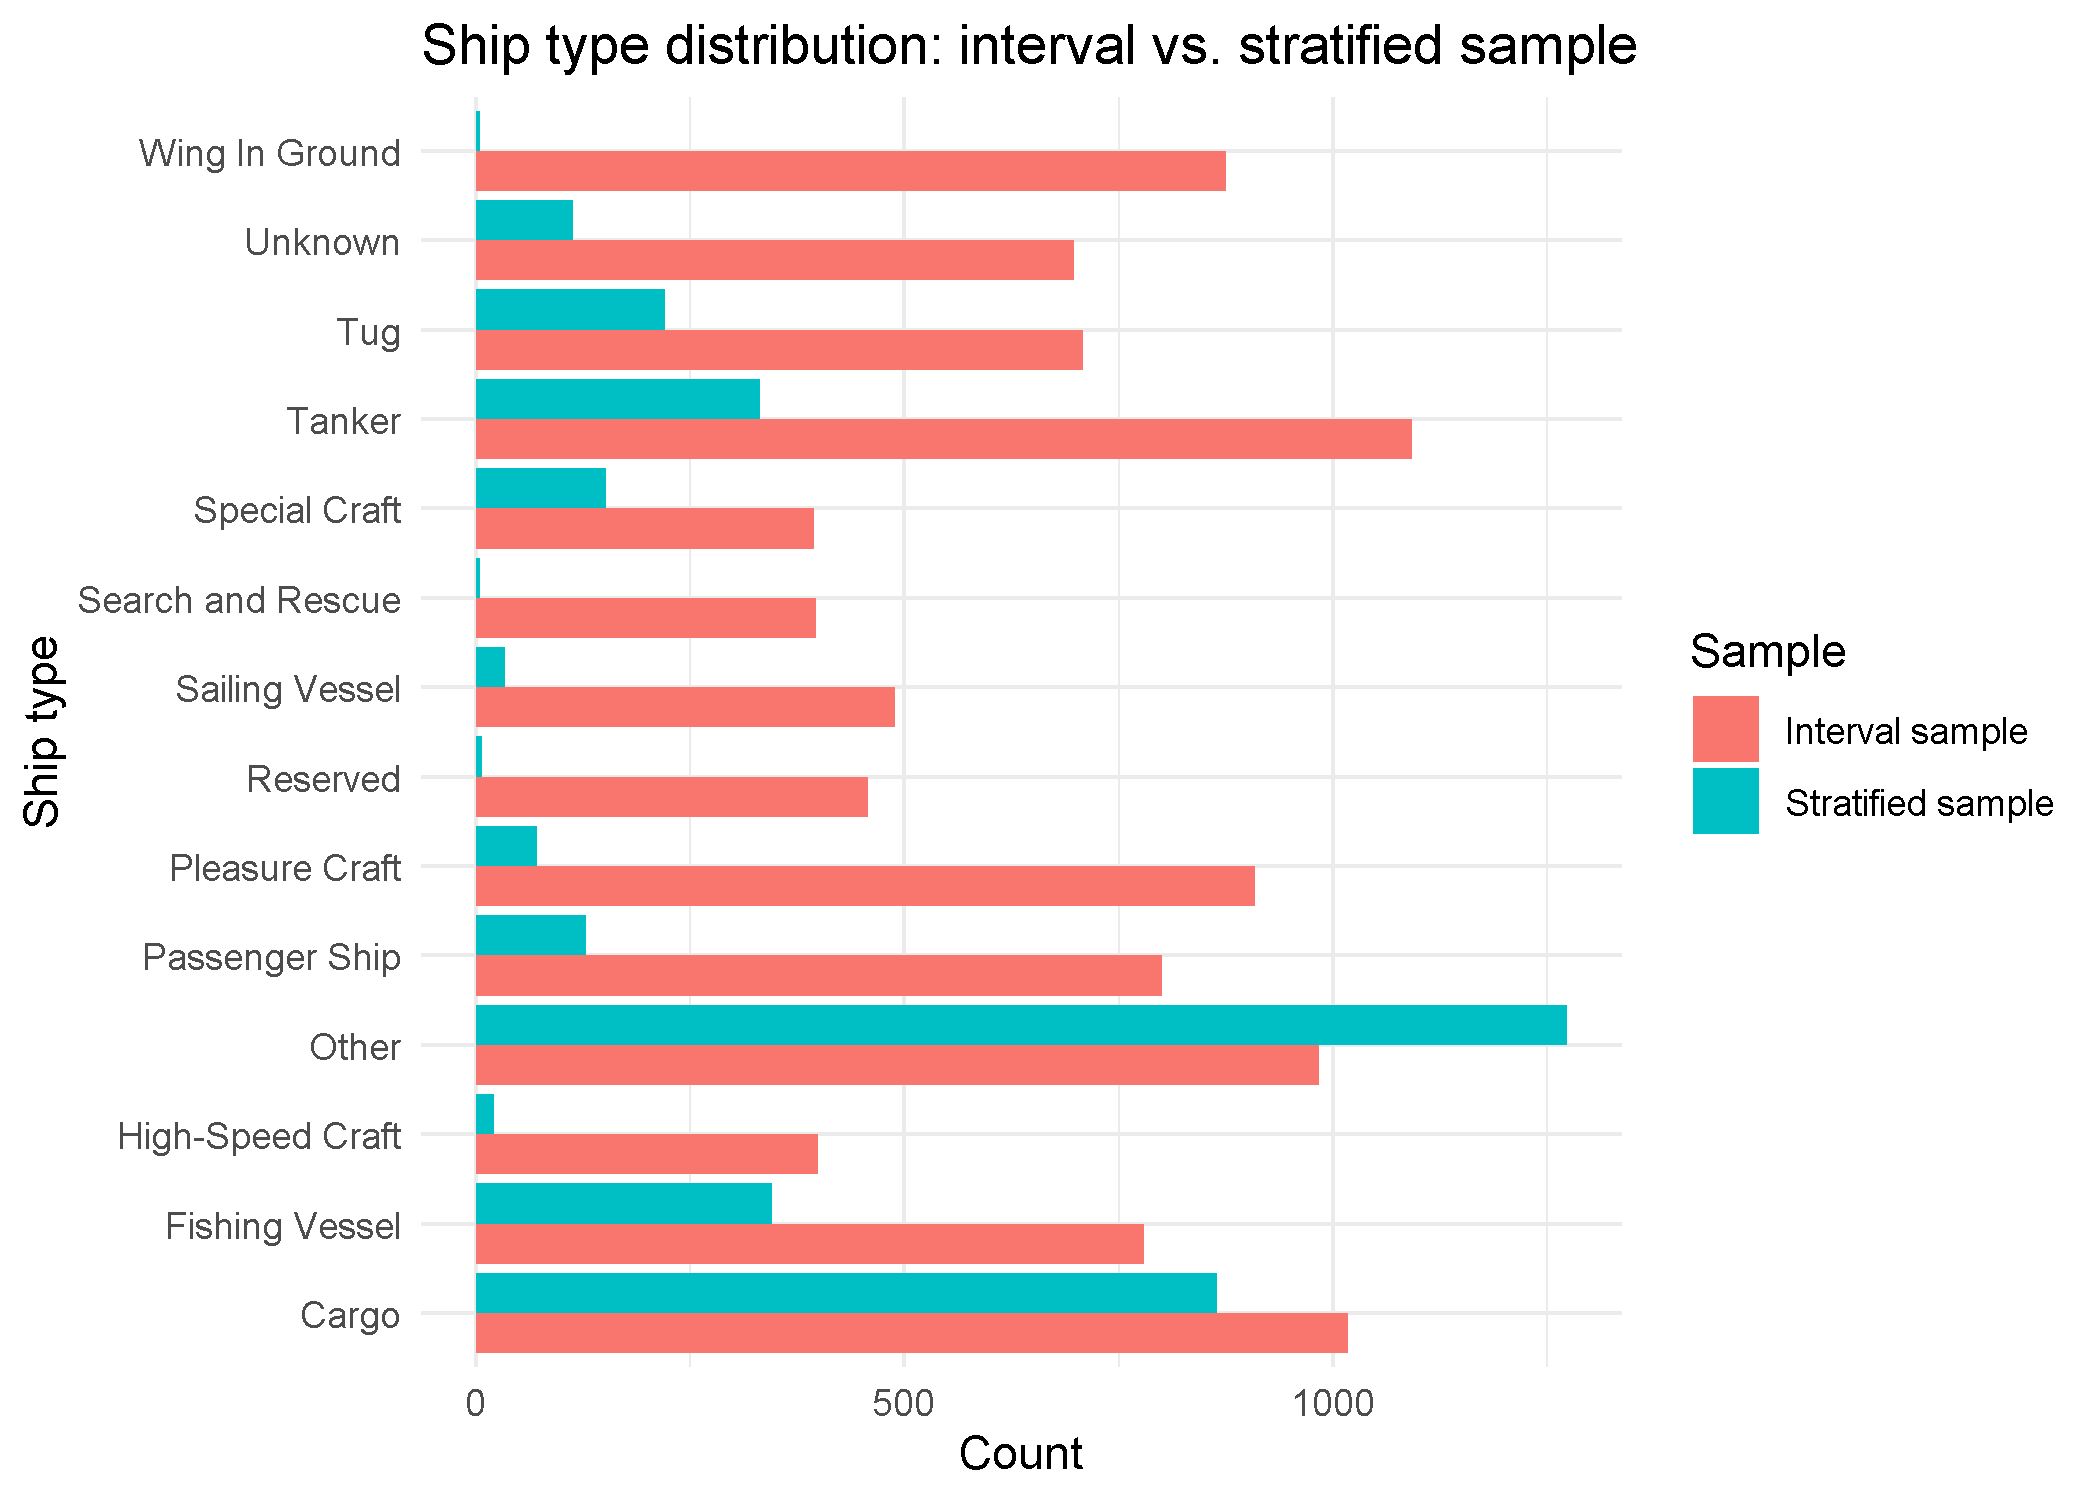
\includegraphics[width=0.85\textwidth]{graphs/compare_ship_type.png}
  \caption{Ship type distribution: interval sample vs.\ stratified sample.
  The stratified sample is constructed to match the population's ship-type
  proportions by design, while the interval sample reflects whichever vessels
  happened to be active during the 100 randomly drawn five-minute windows.}
  \label{fig:cmp-shiptype}
\end{figure}

\begin{figure}[h]
  \centering
  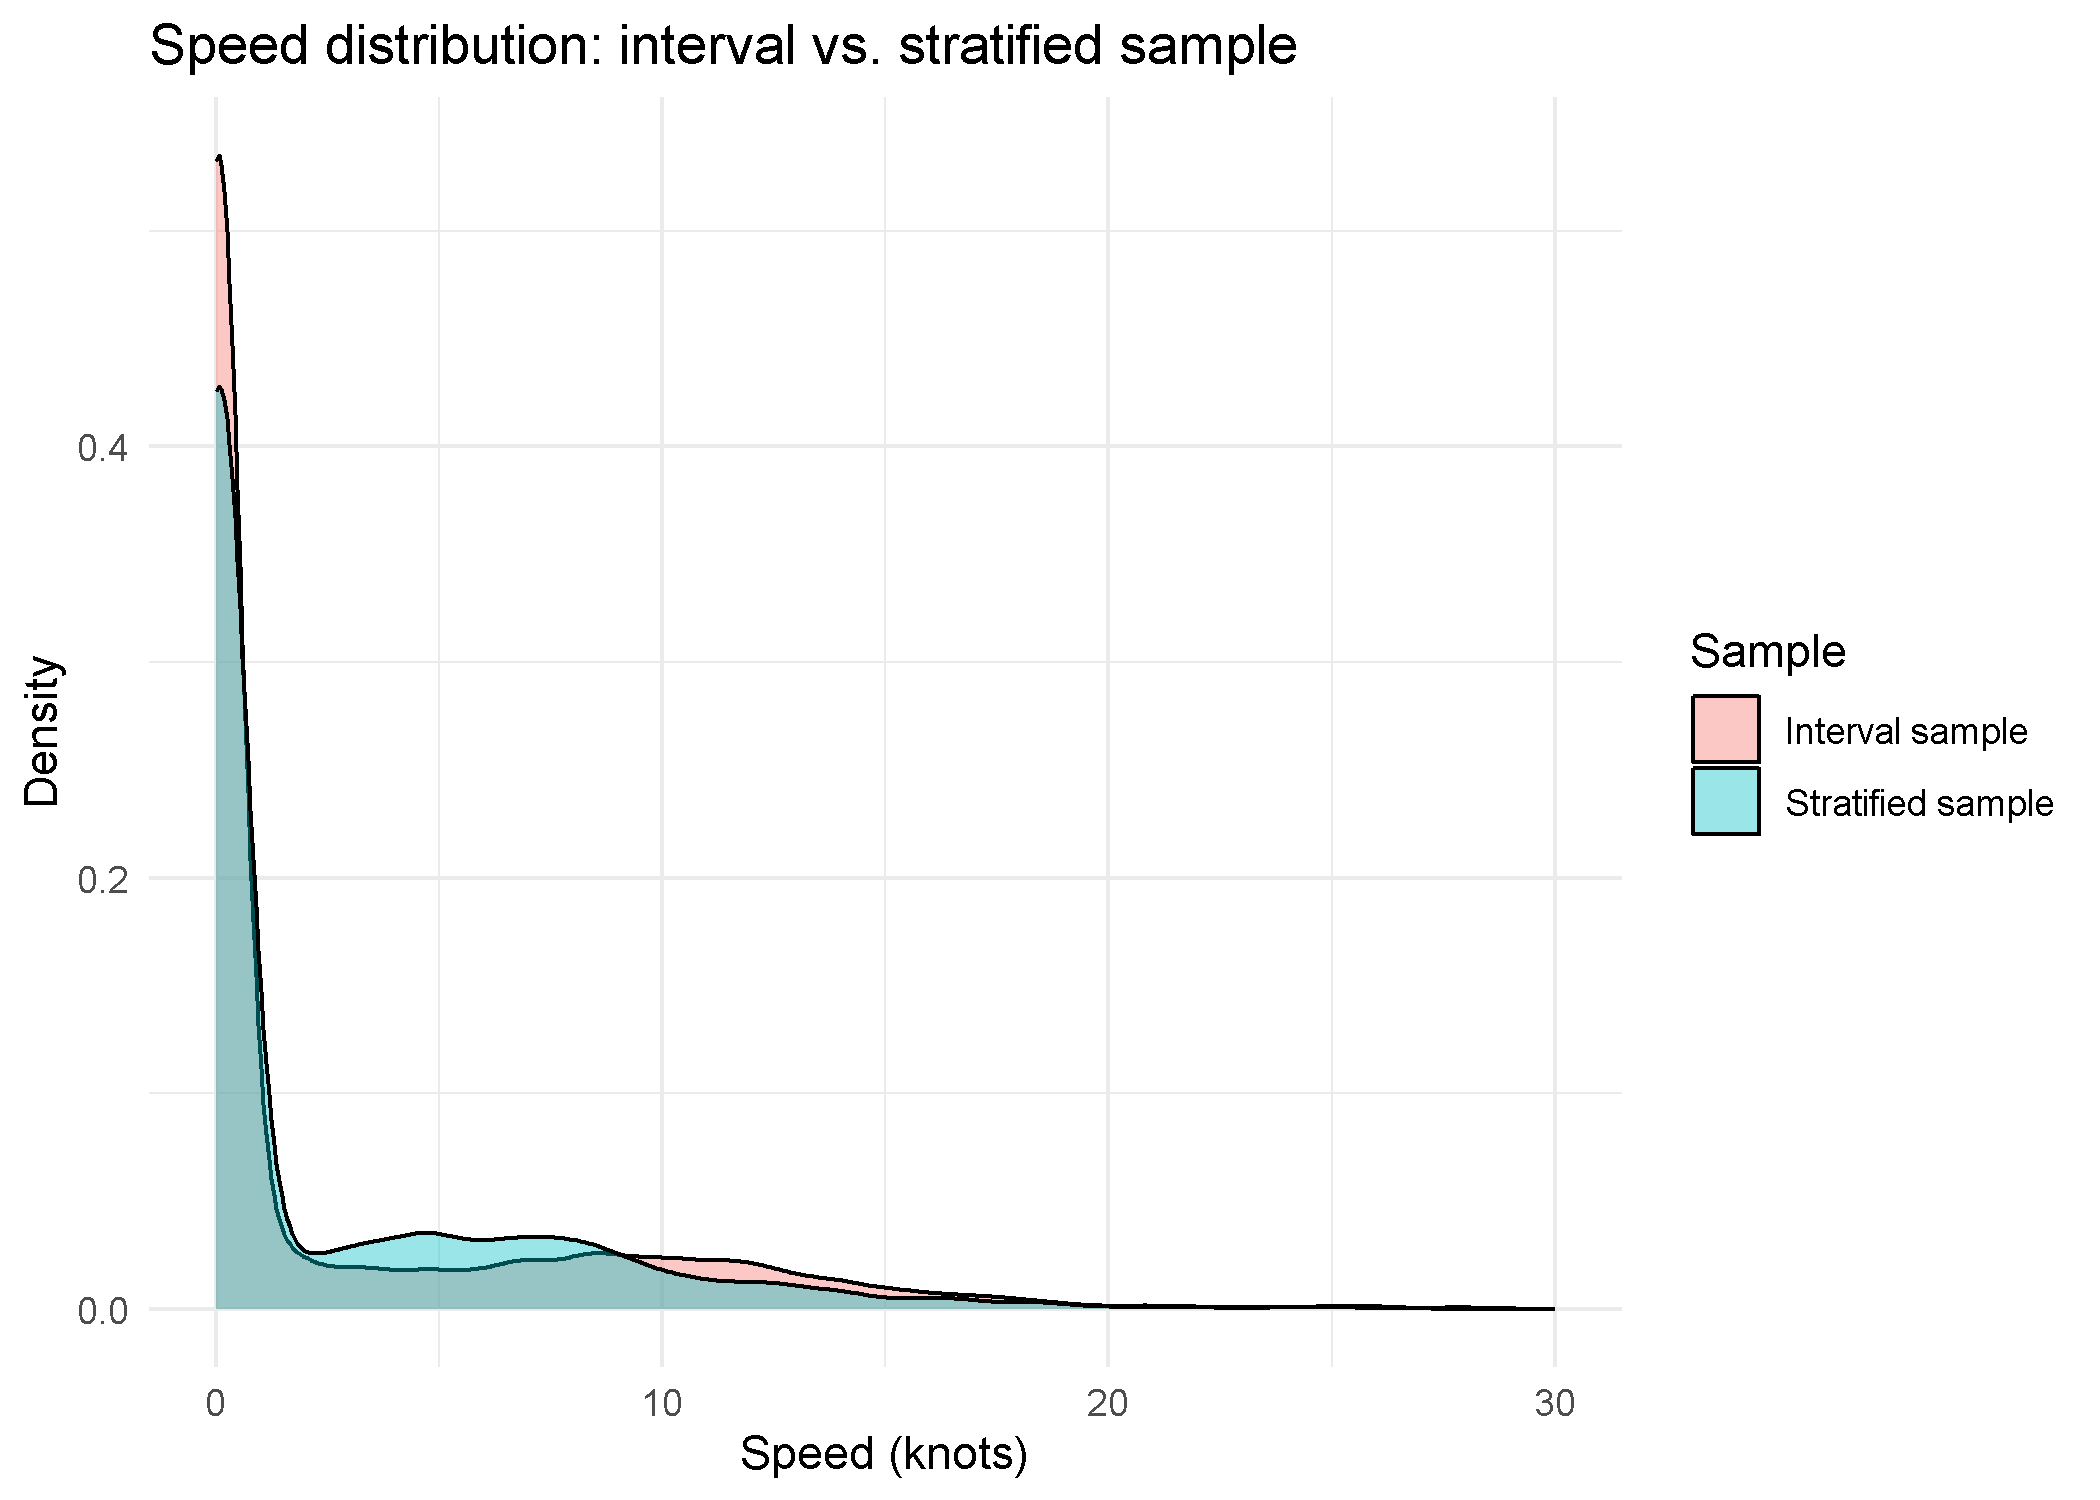
\includegraphics[width=0.85\textwidth]{graphs/compare_speed.png}
  \caption{Speed distribution: interval sample vs.\ stratified sample.}
  \label{fig:cmp-speed}
\end{figure}

\begin{figure}[h]
  \centering
  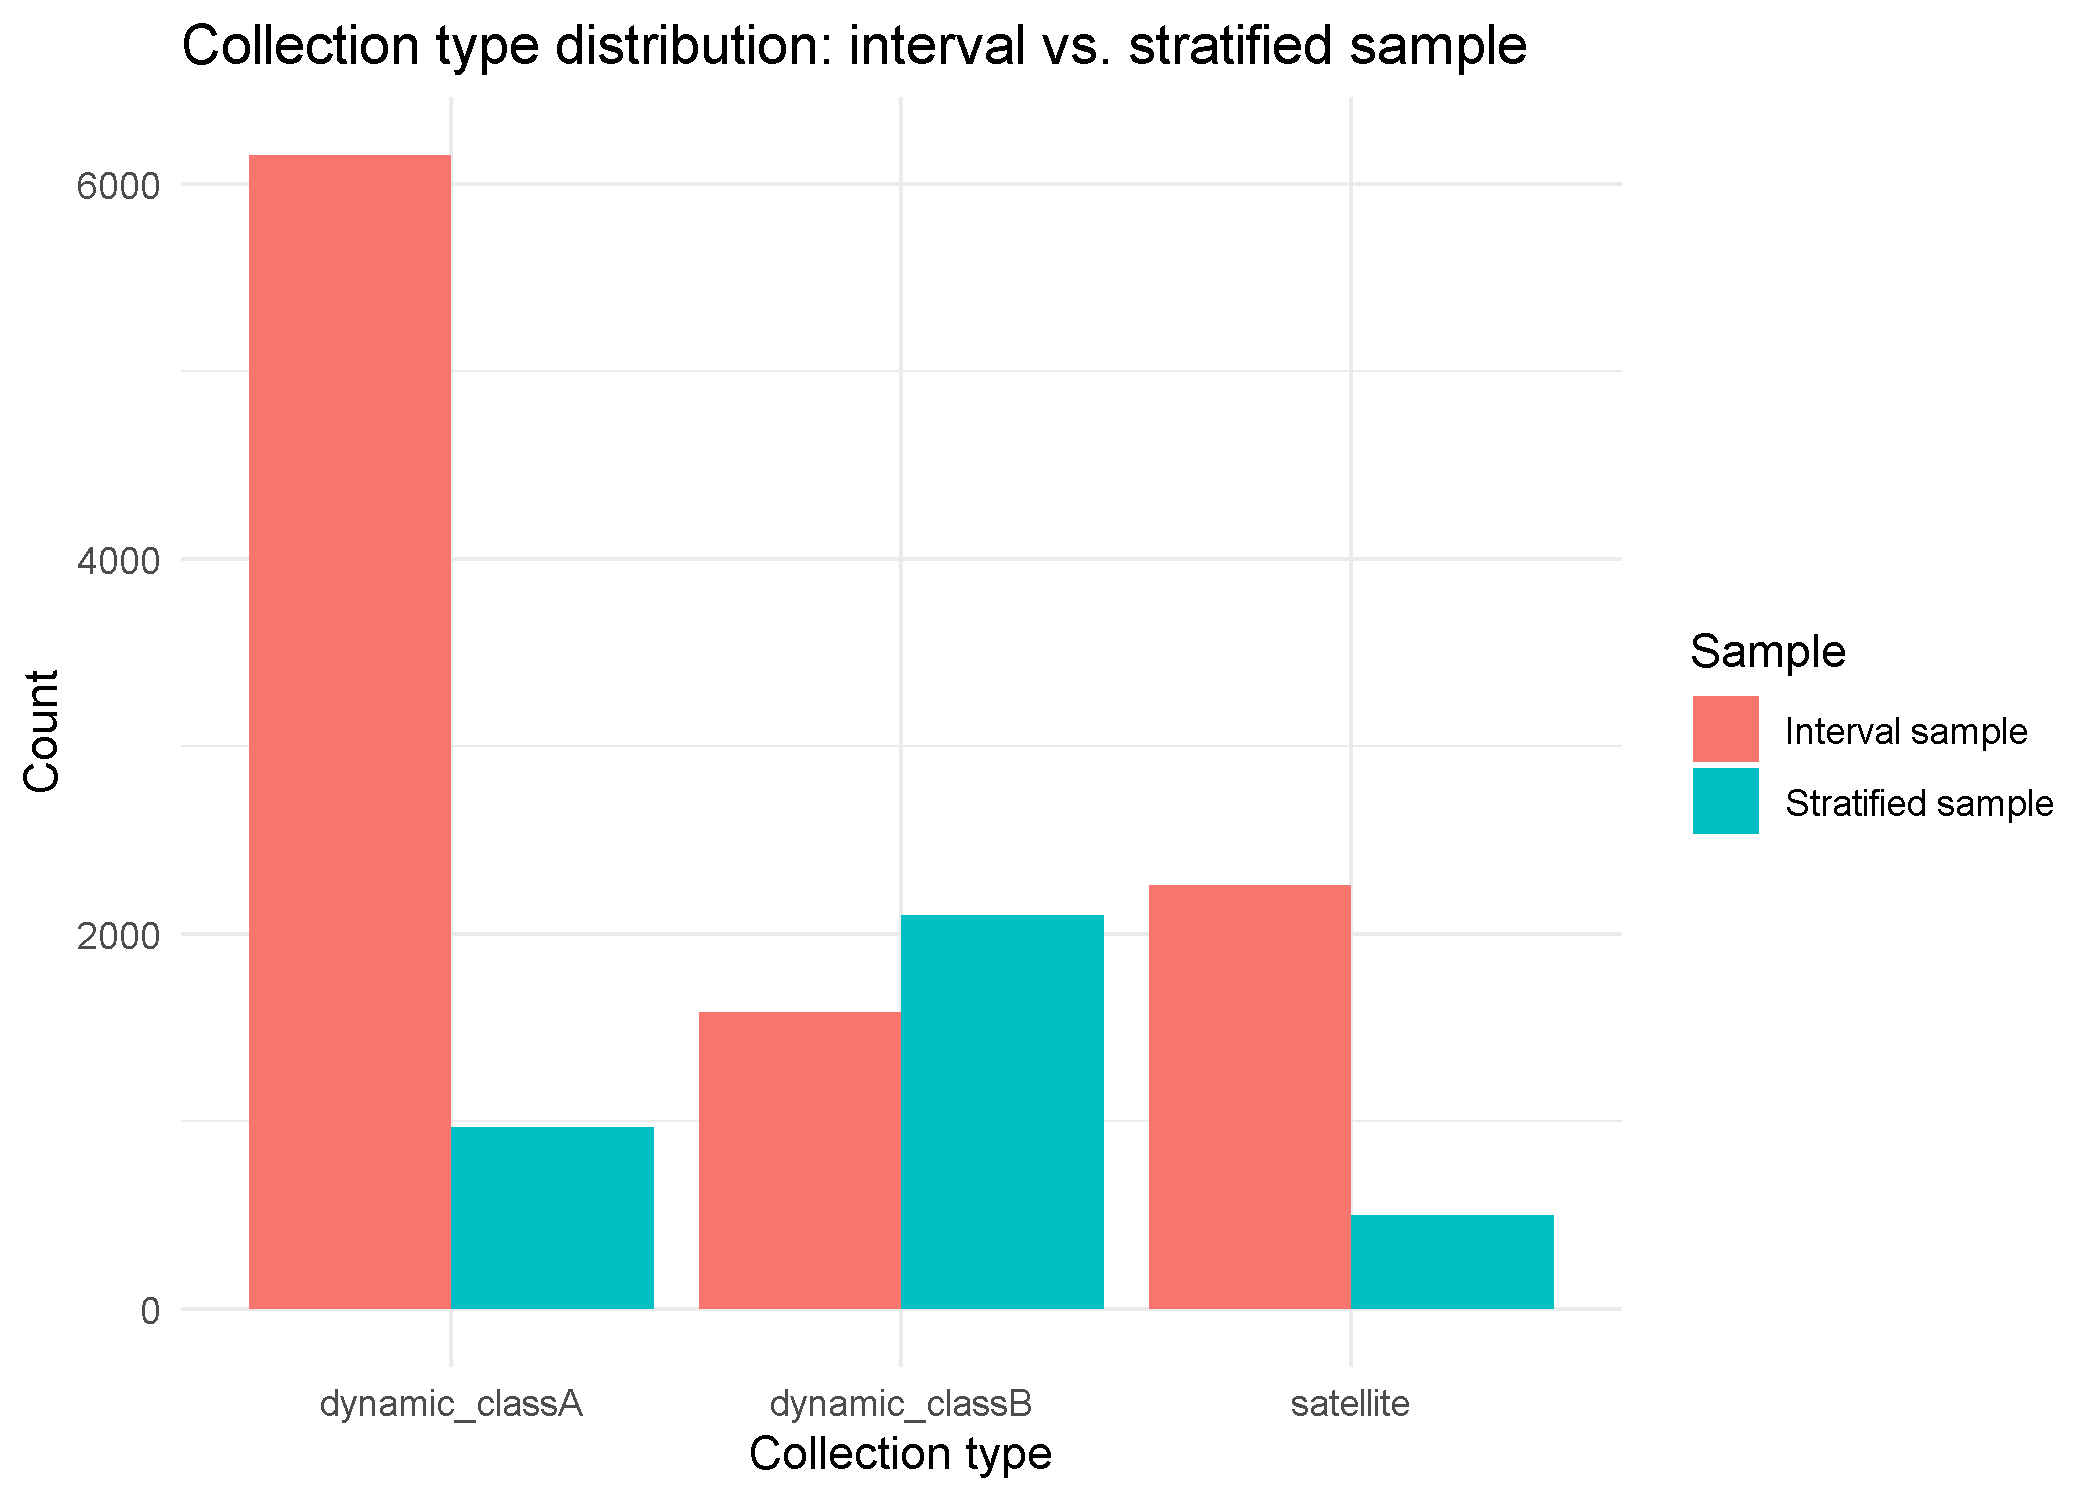
\includegraphics[width=0.85\textwidth]{graphs/compare_collection_type.png}
  \caption{Collection type distribution: interval sample vs.\ stratified sample.}
  \label{fig:cmp-collection}
\end{figure}

The two samples diverge most clearly in \texttt{collection\_type} composition
and in size: the interval sample reached the full 10{,}000-record target,
while the stratified sample fell short (3{,}572 records), since several
(\texttt{ship\_type}, hour) strata could not be fully filled from the
per-hour pool. In the interval sample, \texttt{dynamic\_classA} dominates
(61.5\,\%), whereas \texttt{dynamic\_classB} dominates the stratified sample
(58.7\,\%) -- a direct consequence of how each design pools and subsamples
records. Speed distributions are similar in shape (both peak near 0 knots,
reflecting moored vessels), but the interval sample has a marginally heavier
high-speed tail (mean 3.65 vs.\ 2.90 knots), consistent with the
cluster-sampling bias from Section~4.1, where a few fast-moving vessels can
dominate a randomly drawn five-minute window. For \texttt{ship\_type}, the
stratified sample is proportional to the population by construction, while
the interval sample's ranking is similar but its absolute counts are larger
for almost every category due to its bigger overall size.

\section{Vessel Behaviour}
\label{sec:behaviour}

\subsection{Sample Dashboard}

The 10{,}000-point interval sample was visualised on an interactive
\texttt{leaflet} map (Figure~\ref{fig:dashboard}), with point colour encoding
vessel speed on a continuous (viridis) colour scale: darker (purple) points
indicate near-stationary vessels, while brighter (yellow) points indicate higher
speeds. After removing rows with missing coordinates or speed, the full sample
contains 9{,}625 points; restricting it to \texttt{collection\_type =
"satellite"} observations only leaves 2{,}137 points (22.2\,\% of the full
sample). The geographic extent (minimum/maximum latitude and longitude) is
identical between the two maps, since both contain points near the poles and
near the antimeridian, but the satellite-only map is visibly sparser overall:
with under a quarter of the points spread across the same global extent, the
dense coastal and inland clusters visible in the full map -- which are
dominated by \texttt{dynamic\_classA}/\texttt{dynamic\_classB} (terrestrial)
receptions -- thin out substantially. This is consistent with terrestrial AIS
receivers only covering areas within line-of-sight of the coast, while
satellite AIS additionally captures (at lower temporal resolution) traffic
further offshore that terrestrial stations cannot reach.

\begin{figure}[h]
  \centering
  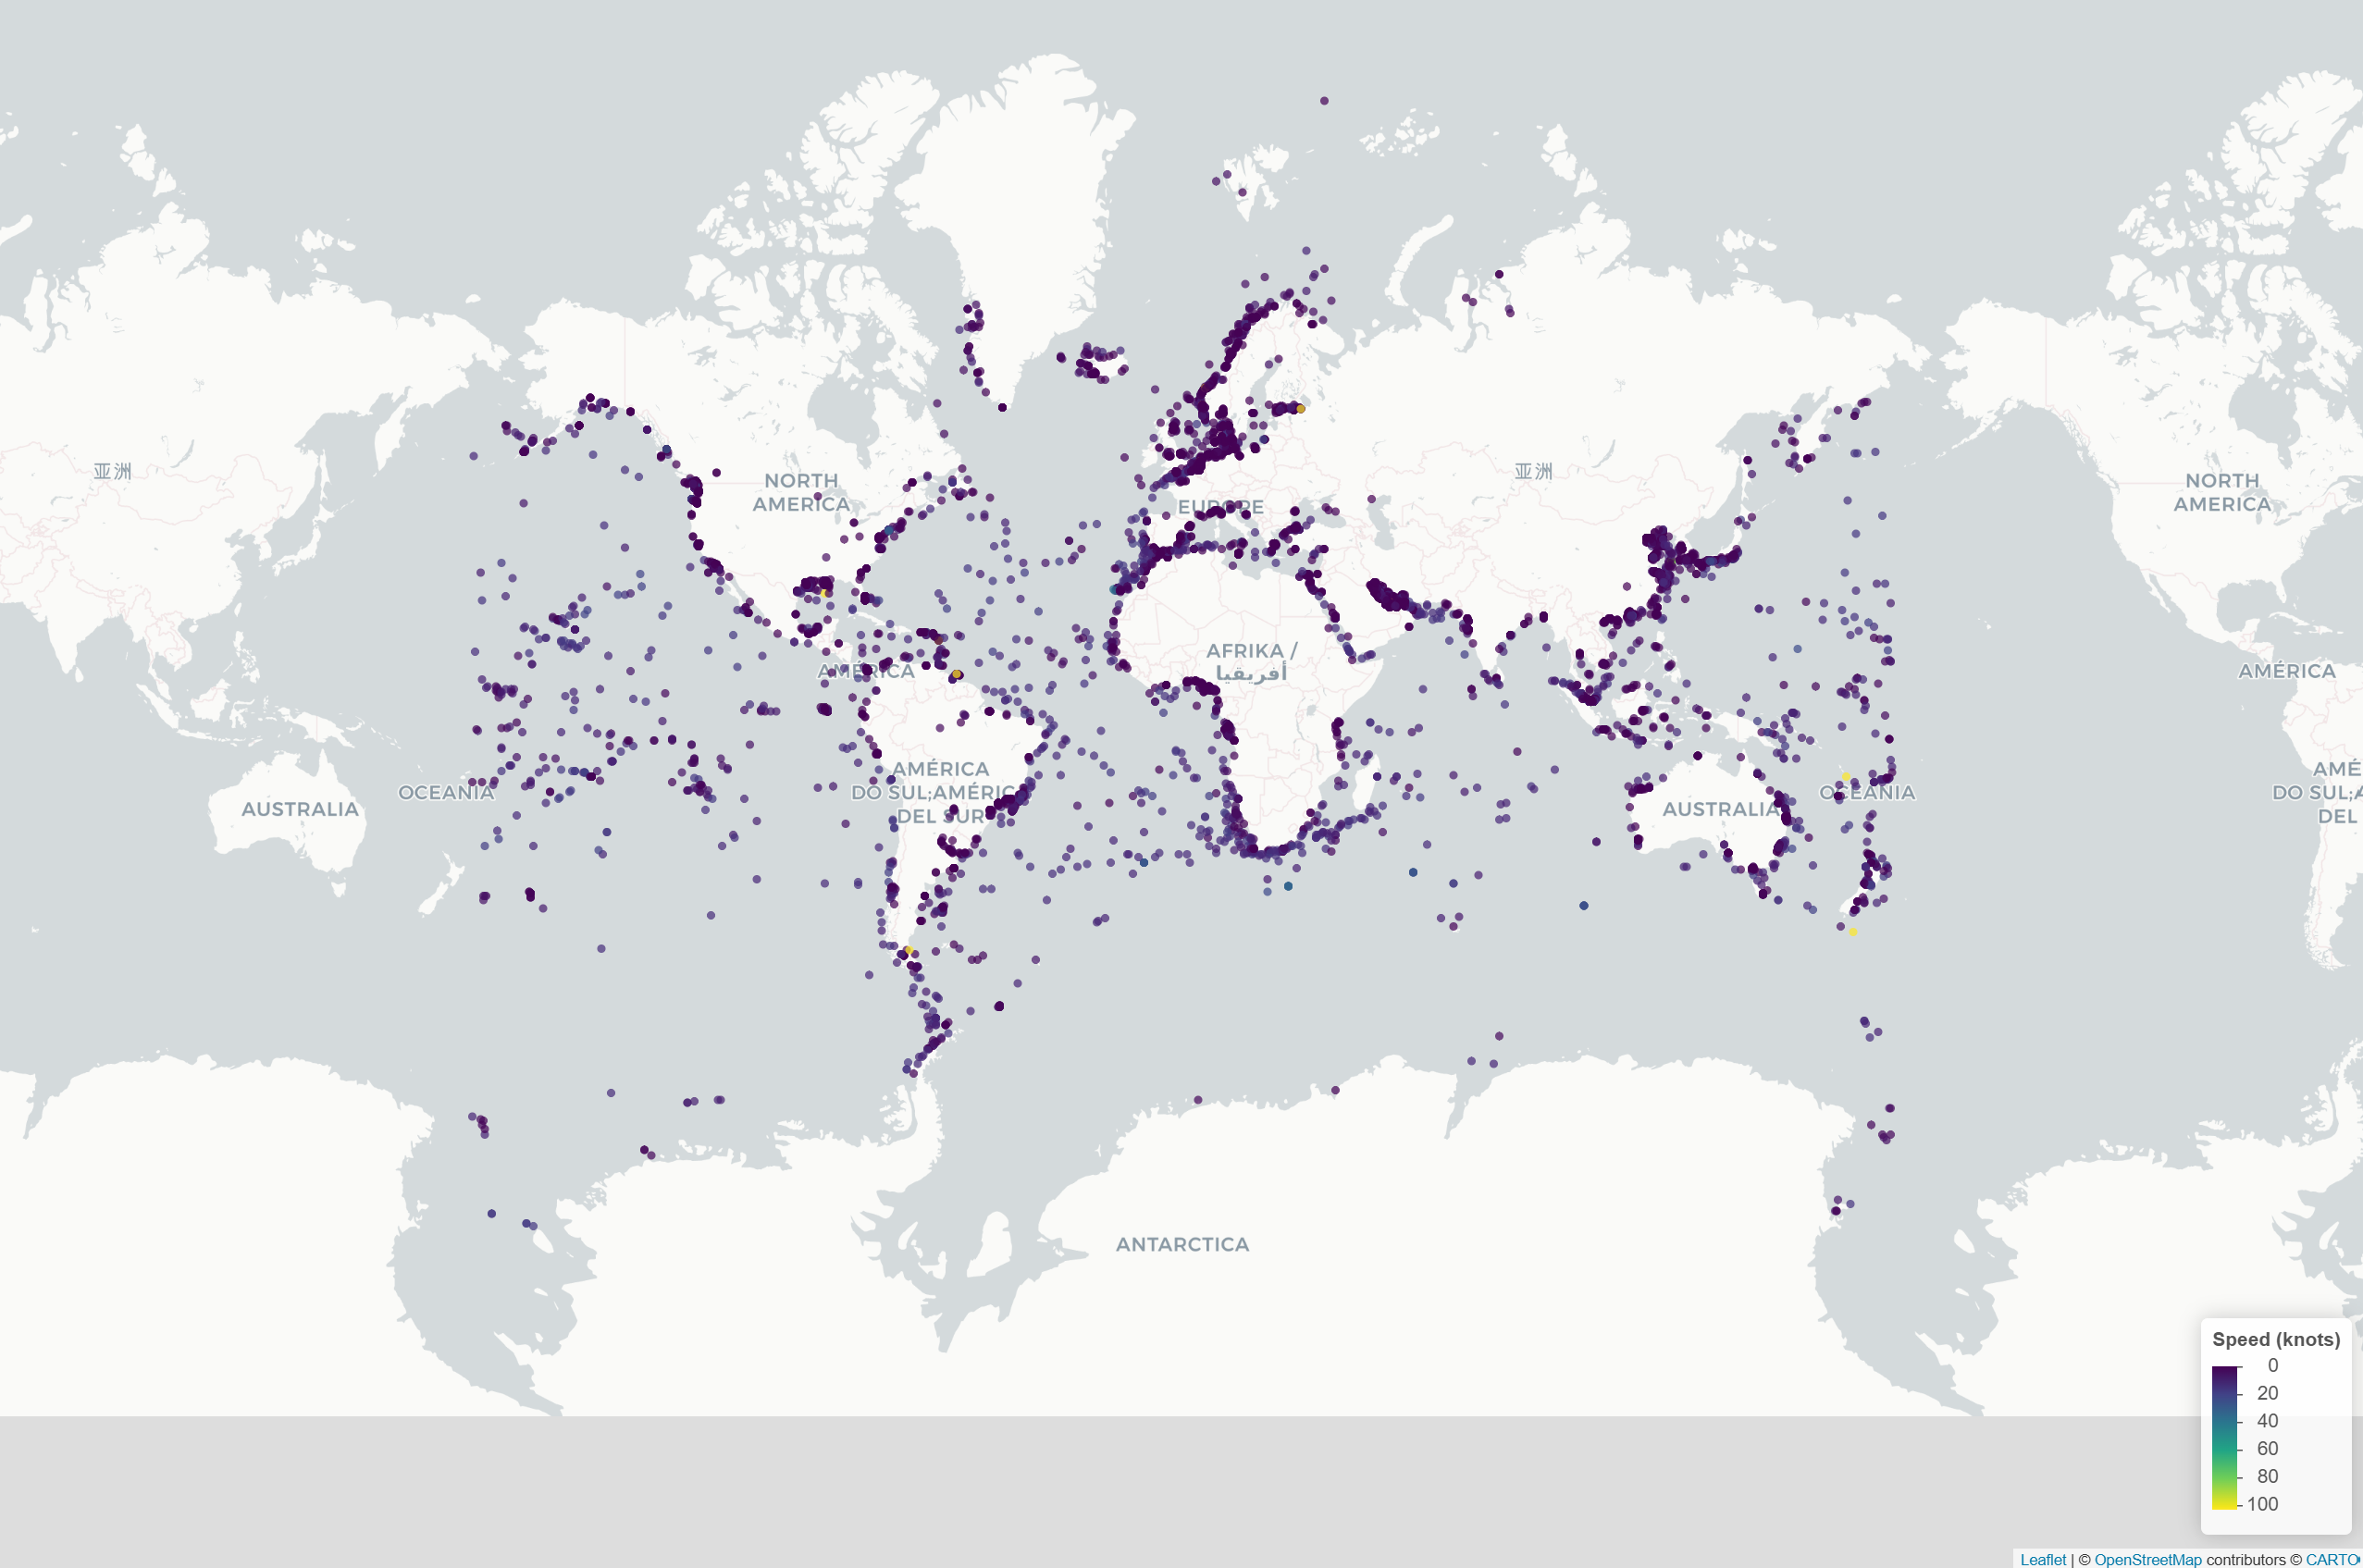
\includegraphics[width=0.9\textwidth]{graphs/sample_dashboard_screenshot.png}
  \caption{Sample dashboard: AIS positions coloured by speed (knots).
  Screenshot of the interactive map produced by \texttt{sample\_dashboard.R}.}
  \label{fig:dashboard}
\end{figure}

\subsection{Individual Vessel Tracks}

\textbf{MMSI 2579999.} As discussed in Section~\ref{sec:limitations}, this MMSI
is too short to be a valid nine-digit vessel identifier and is publicly listed
as an unnamed base station rather than a ship, and separately appears on a
public spoofing-anomaly MMSI list. The associated dynamic records should
therefore be treated as a data-quality artefact rather than genuine vessel
movement. Inspecting a sample of 50 dynamic records confirms this: \texttt{speed}
is missing (\texttt{NA}) for every single record, and the reported positions
jump between widely separated locations -- e.g.\ south-eastern Australia,
the United Kingdom, South Korea, Guinea, Singapore, Norway, Egypt, and
Germany -- within the same few seconds, with several of these locations
recurring repeatedly and near-identically across different timestamps. This
pattern is inconsistent with a single physical vessel and instead suggests
that MMSI 2579999 functions as a fallback or default identifier under which
multiple distinct, genuine transmitters are being recorded simultaneously
(e.g.\ due to misconfigured or factory-default AIS transponders), rather than
representing the movement of one real ship.

\textbf{MMSI 563040400.} Over the queried window,
the vessel's positions are confined to a narrow area near
44.0\textendash44.1\,$^\circ$N, 28.7\textendash28.8\,$^\circ$E -- on the
Romanian Black Sea coast near Constan\c{t}a / the Danube\textendash Black Sea
canal mouth -- rather than showing a long-distance transit. Speed is 0 knots
at the median and at both the first and third quartile (mean 0.34 knots),
indicating that the vessel is stationary or barely moving for the great
majority of the observed records, consistent with time spent moored or
waiting in a harbour/canal area; a maximum speed of 11.7 knots shows that the
vessel does undertake brief, faster manoeuvring or transit phases between
these largely stationary periods.

\subsection{Ship-Lock Events}

A ship lock is expected to leave a distinctive signature in AIS data: speed
drops to near zero for an extended period while the vessel is raised or
lowered, the recorded position stays essentially fixed, the stop typically
lasts on the order of 10--40 minutes, and the local density of AIS observations
is often elevated, since AIS reporting intervals shorten as a vessel's speed and
course-change rate decrease.

We implemented a rule-based detection procedure (\texttt{detect\_lock\_events()}
in \texttt{ais\_dynamic\_individual\_paths.R}) summarised by the following
decision sequence:

\begin{enumerate}[noitemsep]
  \item Sort observations chronologically.
  \item Flag a point as a \emph{candidate} if speed $< 1$ knot.
  \item Merge consecutive candidates into one event if the time gap to the
        previous candidate is $\leq 15$ minutes \emph{and} the spatial distance
        is $\leq 300$\,m.
  \item Keep an event if it lasts at least 5 minutes \emph{or} contains at
        least 4 AIS observations.
  \item For each remaining event, report start time, end time, duration,
        mean location, and the number of observations.
\end{enumerate}

The 1-knot threshold reflects that vessels under power on open water rarely
sustain such low speeds, while a genuine lock passage requires coming to a near
stop; the 300\,m / 15-minute joint condition keeps a single lock chamber
together while preventing two unrelated stops (e.g.\ a lock stop and a much
later anchoring event) from being merged into one event. The final filter
combines two criteria rather than duration alone: in this dataset, several
genuine stops consist of multiple AIS records that all share an identical
\texttt{msg\_timestamp} at to-the-second resolution, so the computed duration
is exactly 0 minutes for those events even though many distinct observations
were recorded at the same location. A duration-only filter would discard
these as noise. Requiring instead at least 4 independent observations as an
alternative qualifying condition is a robust complementary signal of a
genuine stop, since a vessel does not transmit dozens of position reports
without an underlying reason to do so.

Applying this procedure to MMSI 211430830 over 2021-01-17 to 2021-01-20
(Vienna--Linz) yields the events in Table~\ref{tab:locks}.

\begin{table}[h]
  \centering
  \caption{Detected lock passages for MMSI 211430830. Values obtained via
  \texttt{ais\_dynamic\_individual\_paths.R}. Duration is 0 minutes for every
  event because all observations within each event share an identical
  \texttt{msg\_timestamp} (see discussion above); events were nonetheless
  retained because each contains at least 4 independent AIS observations.}
  \label{tab:locks}
  \begin{tabular}{lrrrr}
    \toprule
    Start time (UTC) & Duration (min) & Latitude & Longitude & N obs.\\
    \midrule
    2021-01-18 & 0 & 47.8826 & 17.5411 & 6 \\
    2021-01-18 & 0 & 48.1762 & 16.4789 & 8 \\
    2021-01-18 & 0 & 48.2437 & 16.3857 & 12 \\
    2021-01-19 & 0 & 48.2503 & 14.4317 & 7 \\
    2021-01-19 & 0 & 48.2781 & 14.3494 & 45 \\
    \bottomrule
  \end{tabular}
\end{table}

\begin{figure}[h]
  \centering
  \includegraphics[width=0.9\textwidth]{graphs/vessel_211430830_locks_screenshot.png}
  \caption{Trajectory of MMSI 211430830 with detected ship-lock events
  highlighted in red.}
  \label{fig:locks-map}
\end{figure}

\textbf{Limitations.} Fixed thresholds are not adaptive across vessel types;
GPS/AIS position noise near lock infrastructure can occasionally split one real
event into two; and the heuristic cannot distinguish a lock stop from other
reasons for stopping (bridge waits, anchoring, technical faults) without
external knowledge of lock coordinates. An unsupervised alternative -- for
example clustering jointly on speed, location, and time (e.g.\ DBSCAN), or a
Hidden Markov Model with a latent "stopped" state -- could detect low-speed
regimes without manually chosen thresholds and could be validated against
publicly available coordinates of known Danube locks.

% ============================================================================
% TODO: Section 6 (AIS Traffic Density / Task 5) is OPTIONAL given the 10-hour
% time budget. If you completed Task 5, replace the paragraph below with your
% actual H3-based analysis, tables, and figures (see THAS_Report_Template.pdf
% for the expected structure: river map, percentage on/off river, grouped bar
% chart by ship type, river ranking table, Rhine traffic-density plot).
% If you did NOT complete Task 5, you may shorten this section to a brief,
% honest statement (as below) rather than removing it, since the assignment
% explicitly anticipates that not all teams will complete every 20-point task.
% ============================================================================
\section{AIS Traffic Density on German Rivers}
\label{sec:rivers}

Due to the time constraints of this submission, the H3-based river-matching
analysis (Task 5) was not completed. The general approach would combine
\texttt{rnaturalearth} river geometries with an H3 hexagonal grid index: H3
indices act as keys into a hash table, so that determining whether an AIS point
lies near a river reduces to a constant-time hash lookup rather than a pairwise
distance computation between every AIS point and every river segment -- an
approach that scales far better to the millions of records in
\texttt{ais\_germany}. We focused the available time on Tasks 1--4 and 6--7,
which are documented in full above and in Section~\ref{sec:dashboard}.

\section{Dashboard and Deployment Evidence}
\label{sec:dashboard}

\begin{table}[h]
  \centering
  \caption{Dashboard and deployment evidence.}
  \label{tab:deployment}
  \begin{tabular}{ll}
    \toprule
    Component & Evidence \\
    \midrule
    Static map dashboard & % TODO: URL, e.g. https://<your-server>/sample_points.html
    \TODO{URL or status} \\
    Interactive Shiny application & % TODO: URL, e.g. https://<your-server>/ais_app
    \TODO{URL or status} \\
    \bottomrule
  \end{tabular}
\end{table}

The static dashboard (Section 6 of the assignment) reuses the speed-coloured
leaflet map from Section~\ref{sec:behaviour}, exported as a self-contained HTML
file via \texttt{htmlwidgets::saveWidget()} and served directly by an NGINX
container. The Shiny application (Section 7, Option B) reads a pre-aggregated
CSV (produced once by \texttt{shiny\_data\_prep.R}, rather than querying the API
live on every interaction) and lets the user select an hour, a collection type,
and one or more ship types; after clicking "Refresh plot", it displays the
number of AIS records per minute (0--59) for the selected filters. NGINX
reverse-proxies requests to \texttt{/ais\_app} to the Shiny container, while
\texttt{/sample\_points.html} is served as a static file from the same NGINX
instance.
% TODO: replace with what actually happened on your server, including any
% issues encountered and how they were resolved, e.g.:
\TODO{2-4 sentences documenting your actual deployment: did both components
come up successfully? Any debugging needed (ports, volume mounts, NGINX
location blocks)? Include a screenshot reference if you took one.}

\section{Conclusion}

This report analysed AIS vessel-tracking data exposed through the AIDAHO
PostgREST/TimescaleDB backend, covering database exploration, sampling
strategy design, and individual vessel behaviour analysis. The descriptive
overview (Section~\ref{sec:overview}) showed a database of 228{,}427 distinct
vessels and over 826 million dynamic position messages, dominated by cargo
and fishing vessels under a small number of major flag states -- consistent
with AIS carriage requirements applying primarily to larger commercial
vessels. Comparing an interval-based (cluster) sample against a stratified
sample (Section~\ref{sec:sampling}) illustrated concretely how sampling design
shapes the resulting data: the stratified sample, allocated proportionally to
\texttt{ship\_type}$\times$hour strata, achieved a more population-representative
composition, while the interval sample inherited biases from drawing whole
five-minute clusters at once, particularly toward higher speeds and uneven
\texttt{collection\_type} representation. The vessel-behaviour analysis
(Section~\ref{sec:behaviour}) demonstrated that data-quality screening is a
necessary first step before any AIS analysis -- MMSI 2579999 illustrates how
a single non-standard identifier can silently aggregate unrelated
transmitters -- and that a transparent, rule-based heuristic can recover
meaningful ship-lock events from raw position and speed data, provided the
detection criteria are adapted to the actual resolution of the underlying
timestamps rather than to textbook assumptions about AIS reporting behaviour.

Given the time available for this submission, we prioritised Tasks 1--4 and
6, which are documented in full above, including working, reproducible R
scripts and the resulting data, figures, and tables. The H3-based river
traffic-density analysis (Task 5) was not completed and is documented as
such in Section above rather than represented with placeholder
results.

Beyond the specific numerical results, the project highlighted a broader
methodological point: working against a live, shared production-scale
database surfaces practical constraints -- query cost, response-size limits,
inconsistent timestamp granularity, and ambiguous or non-standard identifiers
-- that do not arise when working with a clean, pre-packaged dataset. Several
of the analytical choices documented in this report (the sample-size
shortfall in Section~\ref{sec:sampling}, the dual duration/observation-count
criterion in the lock-detection function, and the corrected time window for
MMSI 563040400) were arrived at by diagnosing and explaining such
discrepancies rather than assuming the first implementation was correct, which
we consider consistent with the transparent and reproducible approach the
THAS guidelines call for.

\section{Declaration on the Use of AI Tools}
\label{sec:ai-declaration}

% TODO: adapt this to be accurate. A template is provided; do NOT submit a
% statement that does not reflect what you actually did.
We used Claude (Anthropic) to support the structuring of the R scripts (API
helper functions, sampling logic, and the rule-based ship-lock detection
function), to draft the LaTeX report skeleton, and to help interpret the
PostgREST documentation. All numerical results, figures, and tables in this
report were generated by running the submitted R scripts against the live AIS
database, and were checked by us against the underlying data before inclusion.
We did not use AI-generated citations without verifying the original sources,
and we are able to explain and reproduce every part of this submission.

\printbibliography

\appendix
\section{Appendix: Reproducibility and Repository Information}

\subsection{Repository Structure}

\begin{itemize}[noitemsep]
  \item \texttt{00\_docs}: assignment sheet and supporting documents.
  \item \texttt{01\_data}: generated sample data (\texttt{sample\_intervals.csv},
        \texttt{sample\_stratified.csv}) and intermediate data products.
  \item \texttt{02\_code}: analysis scripts (\texttt{R/}) and reusable helper
        functions (\texttt{functions/api\_helpers.R}).
  \item \texttt{03\_report}: this report and all figures (\texttt{graphs/}).
\end{itemize}

\subsection{Execution Order and Reproduction Notes}

Scripts are run from the project root in the following order:
\texttt{02\_overview.R} $\rightarrow$ \texttt{ais\_dynamic\_sample\_points.R}
$\rightarrow$ \texttt{sample\_dashboard.R} $\rightarrow$
\texttt{ais\_dynamic\_individual\_paths.R} $\rightarrow$
\texttt{sample\_html\_dashboard.R} $\rightarrow$ \texttt{shiny\_data\_prep.R}.
Full details are documented in \texttt{README.md}.

\subsection{Software Environment}

\begin{table}[h]
  \centering
  \caption{Software environment used to produce the submitted results.}
  \begin{tabular}{ll}
    \toprule
    Component & Version or description \\
    \midrule
    R version & 4.6.0 \\
    Operating system & Windows 11\\
    \bottomrule
  \end{tabular}
\end{table}

\subsection{Important Submitted Files}

\begin{itemize}[noitemsep]
  \item \texttt{README.md}: instructions for reproducing the analysis.
  \item \texttt{01\_data/sample\_intervals.csv}: interval (cluster) sample.
  \item \texttt{01\_data/sample\_stratified.csv}: stratified sample.
  \item \texttt{03\_report/graphs/}: all figures used in this report.
\end{itemize}

\end{document}